% !TEX root = ../../lectures.tex
\section{First-Order Fermi Mechanism or Diffusive Shock Acceleration}

The mechanism often associated with Fermi is, in fact, the result of the work by several authors, as Krymsky, Bell, Blandford, and Ostriker in the late 1970s~\cite{addref}. 
%
%Krymsky, G. F. Dokl. Akad. Nauk SSSR 243, 1306 (1977). 13. 
%Bell, A. R. M.N.R.A.S. 182, 147 (1978).
%Axford, W. I., Leer, E., and Skadron, G. Proc. 15th ICRC (Plovdiv) XI, 132 (1977). 15. 
%Blandford, R. D. & Ostriker, J. P. Astrophys. J. Lett. 221, L29 (1978).
%
They discovered that \emph{astrophysical shocks} could act as extremely efficient accelerators for cosmic particles, a process now known as \emph{diffusive shock acceleration (DSA)}.

Current observations confirm that particles are indeed accelerated at these shocks, evidenced by the radiation emitted from such regions, typically interpreted as the energy losses of fresh accelerated electrons~\cite{ref}. 

We know at this point that \TODO{(see section)}, in the vicinity of the discontinuity, the upstream region is characterized by fast-moving, cold plasma, whereas the downstream region contains slower, hotter plasma. 
%
The typical shock wave's velocity in the ISM is approximately \( \sim 10^3-10^4 \) km/s, which corresponds to a Mach number of about \( 10^2-10^3 \), placing us firmly in the \emph{strong} shock regime.

The key concept here revolves around how particles perceive the plasma in the context of a shock front. 

From a particle's perspective, the plasma appears to approach at about the shock velocity from both the upstream (\( u \)) and downstream (\( d \)) sides. 
%
Consider a group of particles with energy \( E \) initially located on the \emph{upstream} side of the shock. These particles undergo diffusion through collisions with magnetic turbulence present in the plasma, which tends to isotropize their angular distribution in the frame where the upstream plasma is at rest.
%
Upon crossing the shock to the \emph{downstream} side, these particles encounter magnetic turbulence associated with the downstream plasma. This plasma is moving towards the particles at a velocity \( \sim \frac{3}{4} u_{\rm shock} \) in the same reference frame. If collisions with the downstream plasma further isotropize the particles, then from the particles' viewpoint, they effectively experience a collision with a \emph{cloud} moving towards them (head-on). 
%
Some of these particles will eventually diffuse back to the upstream side of the shock. Upon their return, they perceive the upstream plasma as moving towards them, on average. In the shock frame, the unshocked plasma advances towards the downstream at a speed of \( |u_u - u_d| \sim u_{\rm shock} \), resulting again in a \emph{head-on} cloud collision.
%
There are \emph{never} crossings in which the particles lose energy, and the increment in energy is the same going in both directions. At such, the continual diffusion of particles back and forth across the shock front can significantly accelerate the particles. 

As in both upstream and downstream scenarios, the particles experience head-on collisions, this mechanism will result in a \emph{first-order} Fermi acceleration.

%Therefore, numerous cycles of crossing the shock can significantly accelerate the particles. 
%Scattering ensures that once the particles enter in the upstream or downstream regions there their velocities become isotropically distributed.
%There are never crossings in which the particles lose energy, and the increment in energy is the same going in both directions.

\begin{figure}[t]
\centering
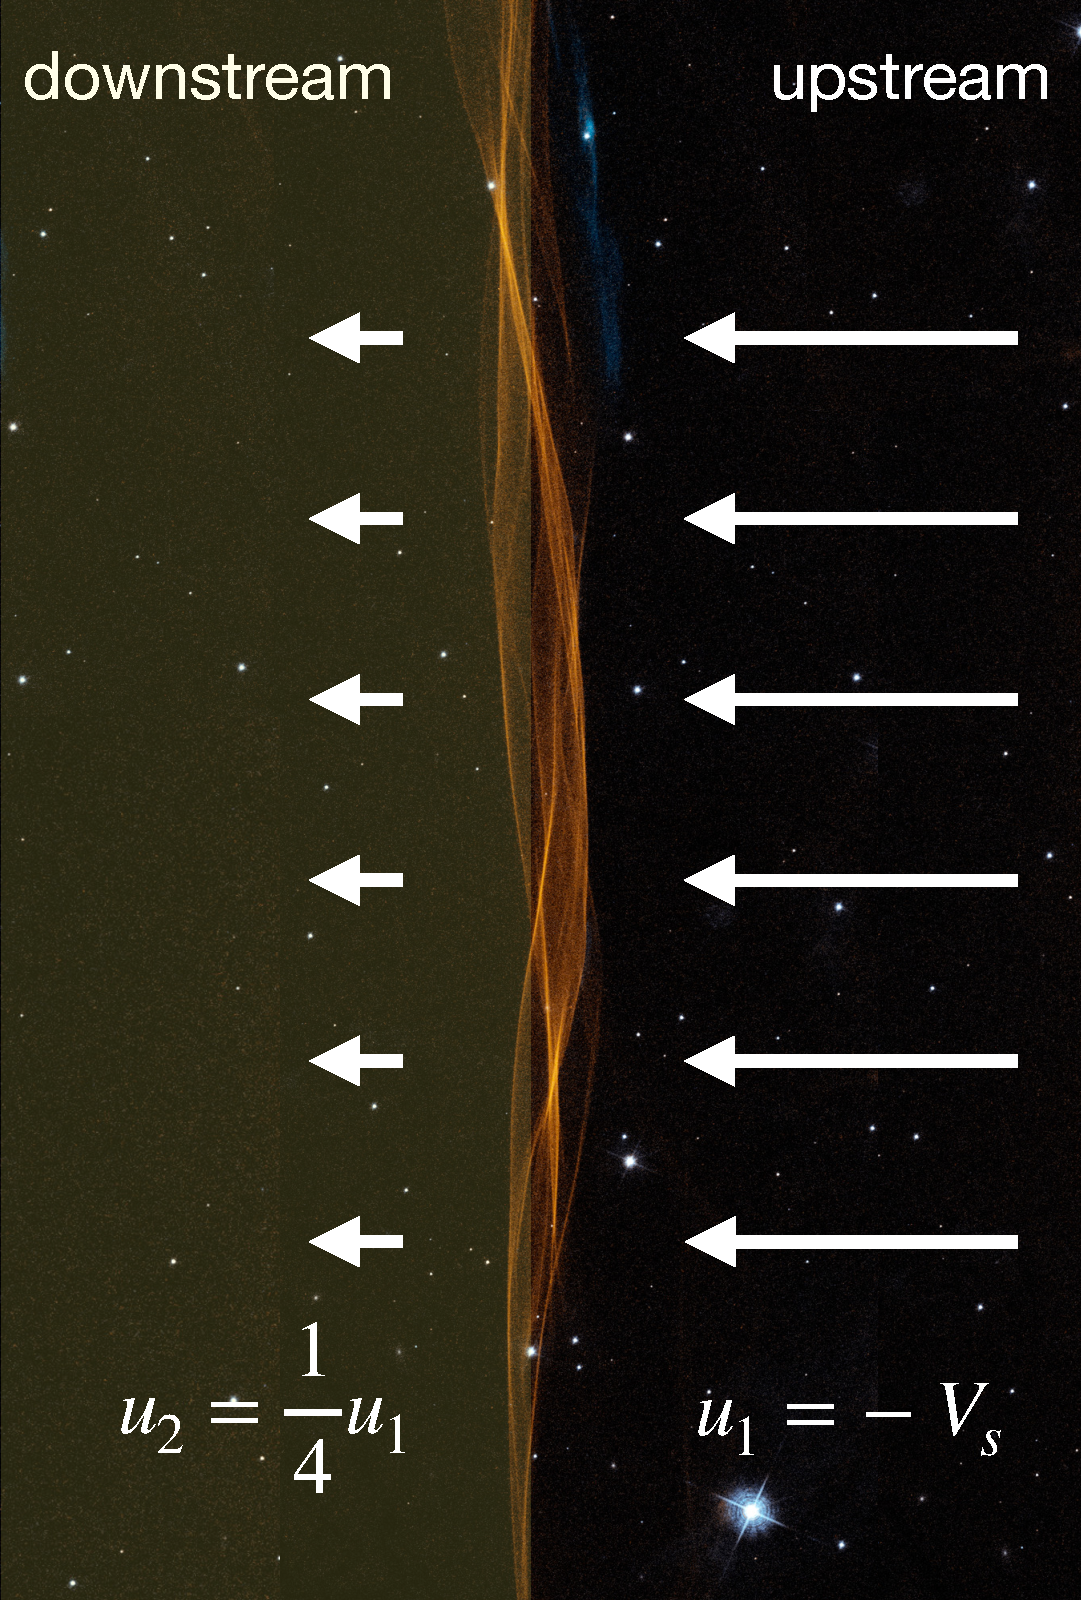
\includegraphics[width=0.31\textwidth]{figures/shockframe0.pdf} 
\hspace{\stretch{1}}
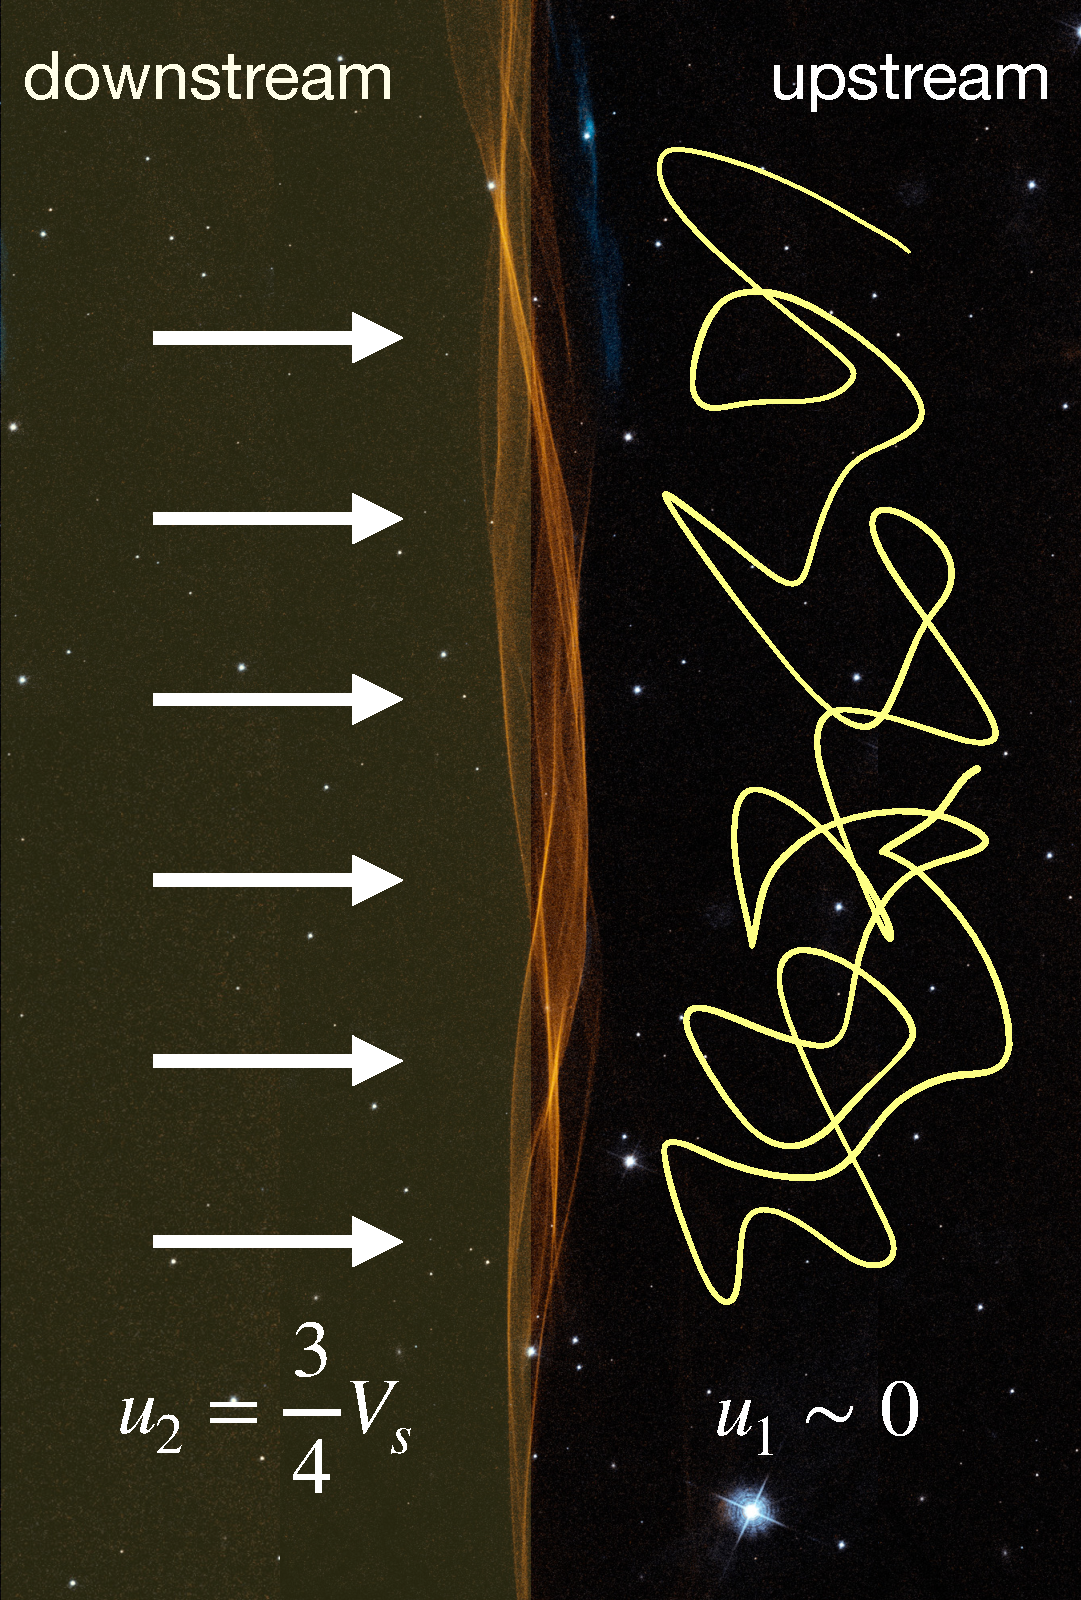
\includegraphics[width=0.31\textwidth]{figures/shockframe1.pdf} 
\hspace{\stretch{1}}
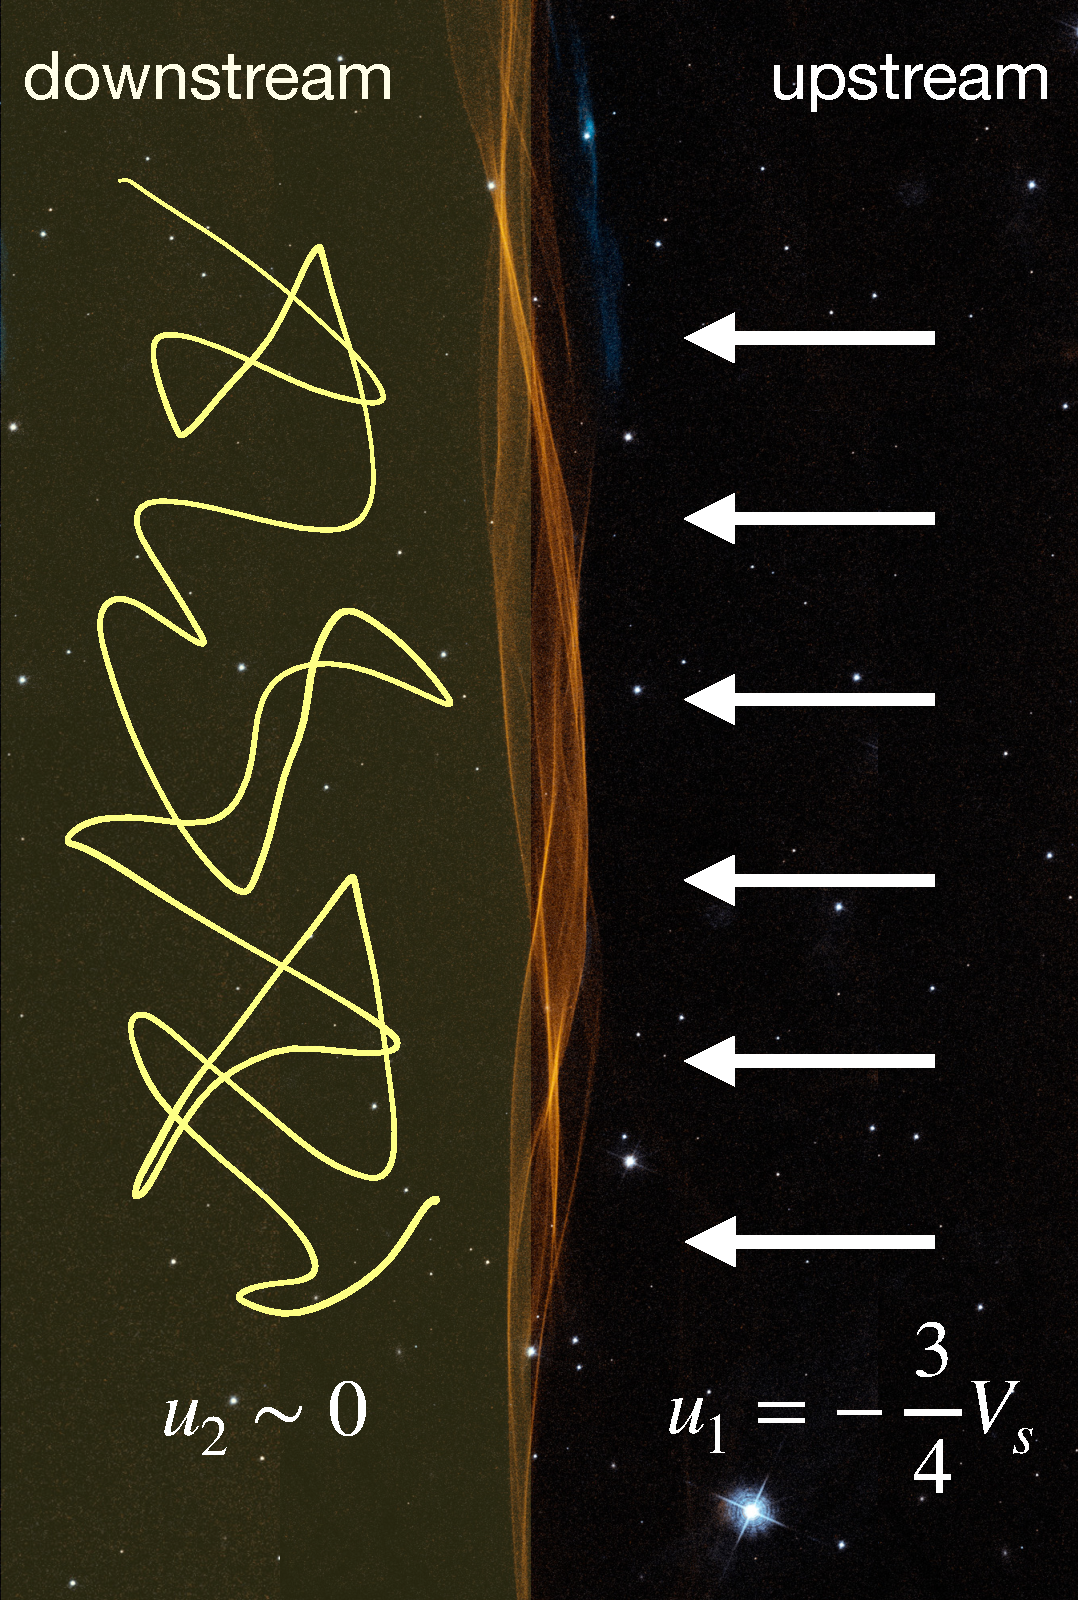
\includegraphics[width=0.31\textwidth]{figures/shockframe2.pdf} 
\caption{Illustration of plasma advection velocities across a shock (moving with velocity \( V_s \) in the Galaxy frame) in three different reference frames. Left panel: the shock is stationary. Center panel: the upstream plasma is stationary. Right panel: the downstream plasma is stationary.}\label{fig:shockframe}
\end{figure}

It is clear from this description that, for this process to occur effectively, particle directions need to be isotropized, which can happen through pitch-angle scattering by MHD waves. The generation of these waves is attributed to large-scale turbulence cascade downstream (injected by the SNR), and upstream by the energetic particles themselves (cosmic-ray streaming).
%
Additionally, it's crucial for particles to have a finite probability of escaping \emph{downstream} to fulfill the conditions of the generalized Fermi acceleration mechanism.

More quantitatively, consider now a particle in the upstream with initial energy \( E_i \). 
%
This particle diffuses and crosses the shock, and its energy in the downstream \( E_i^\prime \) can be calculated using Lorentz transformation:
%
\begin{equation}
E_i^\prime = \gamma E_i \left( 1 + \beta \mu_i \right)
\end{equation}
%
here, \( 0 \le \mu_i \le 1 \) and
%
\begin{equation}
\beta = \frac{u_u - u_d}{c} > 0~.
\end{equation}

The same principle applies to a particle transitioning from downstream to upstream, with the angle \( \mu_f^\prime \) having the opposite sign:
%
\begin{equation}
E_f = \gamma E^\prime_f (1 - \beta \mu_f^\prime)
\end{equation}
here, \( -1 \le \mu_f^\prime \le 0 \).

As a consequence, after completing a cycle (upstream $\rightarrow$ downstream $\rightarrow$ upstream), and assuming \( E^\prime_f \simeq E^\prime_i \), there is an overall gain in energy:
%
\begin{equation}
\frac{\Delta E}{E} = \frac{E_f - E_i}{E_i} = \overbrace{\gamma^2}^{\ge 1} \overbrace{(1 + \beta \mu_i)}^{\ge 1} \overbrace{(1 - \beta \mu_f^\prime)}^{\ge 1} - 1 > 0
\end{equation}

Notice that now, due to the different angular distributions, there are no configurations leading to an energy decrease, and \( \Delta E / E \) is \emph{always positive}.

To compute the mean energy gain over all the possible configurations, we have to compute the probability of a particle encountering the shock front with a specific pitch angle \( \mu \). 

Assuming \( n \) is the number density of isotropically distributed particles due to diffusion, this probability can be derived from the ratio of the flux of particles moving in the direction of \( \mu \) (\( J_\mu = n v \mu \)) to the total flux \( J \):
%
\begin{equation}
J = \int \frac{d\Omega}{4\pi} J_\mu = \frac{n v}{4\pi} \int_0^{2\pi} d\phi \int_0^1 d\mu \mu = \frac{n v}{4}
\end{equation}
%
where we use the information that only those particles with a projected \( \cos \theta > 0 \) will actually cross the shock front.

Therefore, the probability density is given by:
%
\begin{equation}
P(\mu) \propto \frac{n \mu v}{J} = 4 \mu
\end{equation}

To normalize \( P \) as a probability, we impose the condition:
%
\begin{equation}
\int_0^1 d\mu_i P(\mu_i) = 1 \rightarrow P(\mu_i) = 2\mu_i
\end{equation}
%
and
%
\begin{equation}
\int_{-1}^0 d\mu^\prime_f P(\mu^\prime_f) = 1 \rightarrow P(\mu^\prime_f) = -2\mu^\prime_f
\end{equation}

%It is evident that this probability is symmetric in both directions. 

Consequently, the average energy gain can be calculated as follows:
%
\begin{remark}
\begin{equation}\label{eq:firstorderxi}
\left\langle \frac{\Delta E}{E} \right\rangle_{\mu_i,\mu_f^\prime} \!\!\! = \! \int_0^1 \! d\mu_i \int_{-1}^0 \! d\mu^\prime_f \, P(\mu_i)P(\mu_f^\prime)\left[ \gamma^2(1+\beta\mu_i)(1-\beta\mu_f^\prime)-1 \right] 
\oset{\beta \sim 0}{\longrightarrow} \frac{4}{3} \beta 
%= \frac{4}{3} \left(\frac{u_u - u_d}{c} \right)
\end{equation}
\end{remark}

This result implies that the energy gain per cycle is \emph{first order} in $\beta$ as expected, for interstellar shock the resulting energy gain is of the order of \( 10^{-2}-10^{-3} \), which is enormously more than the second order mechanism! 

In assessing the efficiency of the proposed mechanism, we must additionally ensure that particles can effectively cross the shock in both directions. 
%s
In the upstream region, particles, regardless of the diffusion coefficient, will eventually encounter the shock front, which moves towards them at thousands of kilometers per second. Hence, the probability of crossing from upstream to downstream, \( P_{u \rightarrow d} \), is 1. Particles leave the upstream region only when their Larmor radius becomes larger than the accelerator's size or the maximum scale of the upstream turbulence.

In the downstream region, besides diffusion, we must consider that the plasma moves away from the shock, dragging particles with it. This leads to a finite probability of particles not returning to the shock front, finally resulting in a \emph{leakage}. 

To estimate this escape probability, we recall that the particle flux through an infinite planar shock is \( n v / 4 \), assuming efficient isotropization in the upstream. In the shock rest frame, there is a particle flow \( u_d n \) downstream, away from the shock front, which is lost to the acceleration process. Therefore, the escape probability is:
%
\begin{equation}
P_{d \rightarrow \infty} = \frac{u_d n}{n v / 4} \sim \frac{4 u_d}{c}
\end{equation}

The probability of return to the shock front is simply:
%
\begin{equation}\label{eq:pdtou}
P_{d \rightarrow u} = 1 - P_{d \rightarrow \infty} = 1 - \frac{4 u_d}{c}
\end{equation}

With \( u_d / c \sim 10^{-2} \), most particles from the downstream will return to the upstream. This results in a highly efficient first-order Fermi acceleration mechanism with a high probability of completing a cycle.

The existence of a small escape probability is crucial, as it leads to a distribution of energies rather than uniform acceleration. Applying equation~\eqref{eq:gammapescxi}, the slope of the \emph{differential spectrum}\footnote{The differential spectrum \( n(E)dE \) is  the number of particles with energy between \( E \) and \( E + dE \) thus \( E n(E) \propto E^{-\gamma} \)} produced by shock acceleration is given by the fractional energy gain (equation~\ref{eq:firstorderxi}) and the escape probability (equation~\ref{eq:pdtou}):
%
\begin{remark}
\begin{equation}
\gamma \simeq \frac{\frac{4}{3} \beta}{4 \frac{u_d}{c}} + 1 = \frac{3 u_d}{u_u - u_d} + 1 = \frac{r + 2}{r - 1} \rightarrow 2
\end{equation}
\end{remark}

We found that this mechanism results in a \emph{universal} power-law spectrum for strong shocks, as the slope depends only on the compression factor. Worth noticing, the accelerated spectrum is independent of the diffusion coefficient, which in turn depends on the poor-understood microphysics of particle-wave scattering.
%
On the other hand, the acceleration process's efficiency and the potential to accelerate particles to sufficiently high energies dramatically depend on the diffusion coefficient. 

\begin{figure}[t]
\centering
\includegraphics[width=0.6\textwidth]{figures/SNRspectra.pdf} 
\caption{Typical gamma-ray energy spectra for several of the most prominent SNRs. Young SNRs (e.g. Tycho) are shown in cyan. Solid lines show hadronic fits to the data. Adapted from~\cite{Funk2015}.}
\label{fig:snrspectra}
\end{figure}

To estimate the acceleration time, we need to consider the energy gain per crossing and the \emph{time taken for each cycle}.

The total time for a cycle, \( \tau_{\rm cycle} \), is the sum of the time spent in the upstream (\( t_{\rm c,u} \)) and downstream (\( t_{\rm c,d} \)) regions:
\[
\tau_{\rm cycle} = t_{\rm c,u} + t_{\rm c,d}.
\]

For each region, the time spent can be expressed as:
\[
t_{\rm c, i} = \frac{\lambda_i}{\langle v_{x,i} \rangle},
\]
where \( \lambda_i \) is the average distance traveled by a particle in region \( i \) (upstream or downstream), and \( \langle v_{x,i} \rangle \) is the average velocity component along the shock normal.

In the presence of isotropic scattering, the average velocity along the shock normal is given by:
\[
\langle v_{x,i} \rangle = \int_0^1 v_i \mu \, d\mu = \frac{v_i}{2}.
\]

Substituting this into the expression for \( t_{\rm c,i} \), we obtain:
\[
t_{\rm c, i} \sim \frac{2 \lambda_i}{c},
\]
where \( v_i \sim c \) has been assumed for high-energy particles. Thus, the total cycle time becomes:
\[
\tau_{\rm cycle} = \frac{2\lambda_u}{c} + \frac{2\lambda_d}{c}.
\]

The average distance traveled by a particle in each region is determined by diffusion, therefore we write:
\[
\lambda_i \sim \sqrt{2 D_i t_i},
\]
where \( t_i \) is the time the particle spends in region \( i \). This time can be approximated by the time it takes for the advected plasma to catch the particle \( t_i \sim \frac{\lambda_i}{u_i} \), where \( u_i \) is the plasma velocity in the respective region. 

Combining these relations, we have:
\[
\lambda_i \sim \frac{2 D_i}{u_i}.
\]

Substituting \( \lambda_i \) into \( \tau_{\rm cycle} \), we obtain:
\begin{equation}
\tau_{\rm cycle} = \frac{4}{c} \left( \frac{D_u}{u_u} + \frac{D_d}{u_d} \right),
\end{equation}
where \( D_u \) and \( D_d \) are the diffusion coefficients upstream and downstream, respectively.

The characteristic acceleration timescale is then:
%
\begin{remark}
\begin{equation}
\tau_{\text{acc}} = \left( \frac{1}{E} \frac{dE}{dt} \right)^{-1} \sim \left( \frac{\Delta E}{E} \frac{1}{\tau_{\rm cycle}} \right)^{-1} \sim \frac{3}{u_u - u_d} \left( \frac{D_u}{u_u} + \frac{D_d}{u_d} \right) \oset{D_d \ll D_u}{\longrightarrow} 4 \frac{D_u}{u_u^2}
\end{equation}
\end{remark}

To compare this time with the age of the system, we use typical values for the upstream diffusion coefficient and the shock speed of a young SNR. For example, with \( D_u \simeq 10^{28}~\text{cm}^2~\text{s}^{-1} (E/\text{GeV})^{1/2} \) and \( u_u = 10^4 \) km/s, we find:
%
\begin{equation}
\tau_{\text{acc}} \simeq 1.3~\text{kyr}~\left( \frac{E}{\text{GeV}} \right)^{1/2} 
\end{equation}

However, observations of particles accelerated up to 100 TeV (see figure~\ref{fig:snrspectra}) in events like Tycho's supernova (age \( \sim 500 \) years) suggest that our estimates are off by orders of magnitude! Reconciling this discrepancy requires \emph{reducing} the diffusion coefficient in the upstream, possibly through cosmic-ray induced plasma instabilities. This leads to an inherently non-linear problem, underscoring the complexity of particle acceleration in astrophysical shocks.